\documentclass[iop]{emulateapj}
\usepackage[latin1]{inputenc}
\usepackage{amsmath}
\usepackage{amsfonts}
\usepackage{amssymb}
\usepackage{graphicx}
\usepackage{tikz}
\usepackage{float}

\usepackage{hyperref}
\usepackage[nolist]{acronym}


\begin{document}
	
	\title{Hyperbolic Heat Conduction Using First-Order Explict Finite Difference}
	\author{Roy Smart}
	%\author{Dana Longcope}
	\affil{Department of Physics, Montana State University, Bozeman MT, 59717, USA}
	
	\begin{abstract}
		
	\end{abstract}
	
	\section{Introduction}
	
		\noindent
		Heat conduction is an crucial process in \ac{MHD} simulations of the solar atmosphere because as the temperature rises to a MK in the solar corona, it becomes the dominant term in the energy equation \citep{gudiksen_11}.
			As a result, heat conduction is important for both controlling the temperature and density of the corona and regulating the height of the transition region \citep{bingert_11}.
			However, an accurate treatment of heat conduction presents several numerical challenges, some of which will be discussed in this study.
			
		Many current comprehensive models of the solar atmosphere such as those by \cite{gudiksen_05} and \cite{A} use \ac{EFD} methods to solve the \ac{MHD} equations since these methods are better suited to \ac{MPP} architectures.
			Since running simulations on \ac{MPP} architecture is an important goal for future work, we will only consider modeling heat conduction using \ac{EFD} methods.
			Of particular importance to \ac{EFD} simulations is the determination of the maximum timestep size, i.e. the minimum temporal resolution of the simulation.
			Rigorously deriving the maximum timestep will be an important facet of this work and will be studied in detail.
		
		This work will focus on modeling heat conduction only, no other terms from the fluid equations will be considered.
			However, we will consider two models of heat conduction, the first being the classic model of diffusion which is a parabolic \ac{PDE}.
			The second model we will investigate will involve adding an additional term to the parabolic model which will transform it into a hyperbolic \ac{PDE}.
			This hyperbolic model was recently used by \cite{A} in the MURaM comprehensive model of the solar atmosphere and was shown to be much more computationally efficient than a corresponding parabolic solution.
			The main goal of this work is to recreate the results of \cite{A} using first-order \ac{EFD} and to ascertain whether there is any performance benefit to be offered using the more complex hyperbolic formulation.
		
	
	
	\section{Background}
		\subsection{Classification of Second-order PDEs}
			Second-order PDEs are organized into groups known as parabolic, hyperbolic and elliptic.
				This classification describes how a disturbance (information) propagates throughout the domain of a \ac{PDE}.
				To understand the mathematical definition of these groups, we start by defining a general second-order \ac{PDE} with two independent variables, $x$ and $t$,
				\begin{align}
					A \partial_{xx} \psi + 2 B \partial_{xt} \psi + C \partial_{tt} \psi + D \partial_x \psi + E \partial_t \psi = 0 \label{gen_pde}
				\end{align}
				where $\partial_y = \partial / \partial y$, $\partial_{yy} = \partial^2 / \partial y^2$, etc.
				The classification of a second-order \ac{PDE} involves only the coefficients $A$, $B$ and $C$ of Equation \ref{gen_pde}.
				
			Hyperbolic \acp{PDE} are defined by the relation 
				\begin{align}
					B^2 - AC > 0.
				\end{align}
				These PDEs are the simplest to understand, since they have properties we have come to expect from the physical world, namely finite information travel time.
				A disturbance in the solution of a hyperbolic PDE can only influence the solution in a ``light cone'' centered around the disturbance.
				The wave equation is a common prototype for this class of PDE.
				
			Parabolic \acp{PDE} are defined by a similar relation
				\begin{align}
					B^2 - AC = 0.
				\end{align}
				In contrast to the hyperbolic case, this type of PDE has infinite information travel time.
				As an example consider a dirac delta function at $t=0$. 
				Under a parabolic PDE, this delta function will become a gaussian with tails extending to infinity at the very next instant, $t>0$.
				The heat equation is a simple prototype for this class of PDE.
				
			Elliptic \acp{PDE} won't be considered in this work, but the definition is easy to guess considering the last two definitions.
				
				
				
		\subsection{Parabolic Heat Conduction}
		
			Parabolic heat conduction is often known simply as the heat equation and is given in one dimension as
			\begin{equation} \label{par}
				\frac{\partial T}{\partial t} - \kappa \frac{\partial^2 T}{\partial x^2} = 0
			\end{equation}
			where $T$ is the temperature, $x$ is a spatial variable, $t$ is time, and $\kappa$ is the thermal diffusivity.
			Take note that Equation \ref{par} is parabolic since $B$ and $C$ are equal to zero.
			
			In numerical solutions, we often prefer considering systems of first-order differential equations.
			The heat equation can be transformed into a system of first-order equations like
			\begin{gather}
				q = -\kappa \frac{\partial T}{\partial x} \label{flux_p} \\
				\frac{\partial T}{\partial t} = -\frac{\partial q}{\partial x} \label{temp_p} 
			\end{gather}
			where we have introduced a new variable $q$ that we interpret as the heat flux using dimensional analysis.
			Equation \ref{flux_p} will be known as the parabolic flux equation, and Equation \ref{temp_p} will be known as the parabolic temperature equation.
			The system formed by the flux and temperature equations will be known as the parabolic heat conduction system, or just the parabolic system.
			
			We will use both Equation \ref{par} and the parabolic system often in this work, please note that they only mean the same thing if the thermal diffusivity is constant.
		
		\subsection{Hyperbolic Heat Conduction}
		
			Hyperbolic heat conduction equations have been proposed by a number of researchers in astrophysics \citep{snodin_06} and solar physics \citep{A}.
				As has been discussed earlier, this work is following the procedure detailed in \cite{A}.
			
				Their approach adds an extra term to the flux equation that is proportional to the time derivative of heat flux.
				\begin{gather}
					\tau \frac{\partial q}{\partial t} + q = -\kappa \frac{\partial T}{\partial x} \label{flux}\\
					\frac{\partial T}{\partial t} = -\frac{\partial q}{\partial x} \label{temp}
				\end{gather}
				where $\tau$ is known as the damping timescale and is an unknown parameter. 
				Similar to the parabolic case, Equation \ref{flux} is known as the hyperbolic flux equation, Equation \ref{temp} is known as the hyperbolic temperature equation, and the system is known as the hyperbolic system.
				
				If we assume that $\kappa$ and $\tau$ are constants, we can express Equation \ref{flux} as a single second-order equation by taking a spatial derivative and plugging in Equation \ref{temp}.
				\begin{align}
					& \frac{\partial}{\partial x} \left( \tau \frac{\partial q}{\partial t} \right) + \frac{\partial q}{\partial x} = - \frac{\partial}{\partial x} \left( \kappa \frac{\partial T}{\partial x} \right) \\
					\Rightarrow \quad & \tau \frac{\partial}{\partial t} \frac{\partial q}{\partial x} + \frac{\partial q}{\partial x} = -\kappa \frac{\partial^2 T}{\partial x^2} \\
					\Rightarrow \quad & \tau \frac{\partial^2 T}{\partial t^2} +  \frac{\partial T}{\partial t} - \kappa \frac{\partial^2 T}{\partial x^2} = 0 \label{wave}
				\end{align}
				The above equation is a linear, damped wave equation in temperature. Notice that $A > 0$, $B = 0$, and $C < 0$, so that $B^2 - A C$ is positive and the equation is hyperbolic.	
				While the solar atmosphere has a temperature-dependent thermal diffusivity $\kappa$, Equation \ref{wave} will still be useful for examining the linear behavior of the hyperbolic system.
		
				If we divide Equation \ref{wave} by $\tau$, we can see that the wave speed of this PDE is 
				\begin{align}
					c = \sqrt{\frac{\kappa}{\tau}} \label{vp}
				\end{align}
				In \cite{A}, they assume $c$ to be a constant, proportial to the ratio of the grid size to the timestep size,
				\begin{align}
					c = f \frac{\Delta x}{\Delta t} \label{v},
				\end{align}
				where $f$ is known as the Courant number and will be discussed in Section \ref{vnsa_sec}.
				They also use the Spitzer form of thermal conduction \citep{spitzer_62}, 
				\begin{align}
					\kappa = T^{5/2}
				\end{align}
				where we are adopting some interesting unit system that makes a scaling constant (which might be named $\kappa_0$) unnecessary.
				
				The above equations provide enough information to solve for the damping timescale, $\tau$. Solving Equation \ref{vp} for $\tau$ gives
				\begin{align}
					\tau = \frac{\kappa}{c^2} = \frac{\kappa \Delta t^2}{f^2 \Delta x^2}.
				\end{align}
				where we have applied Equation \ref{v}. 
				This formulation ensures that the wave speed does not exceed the maximum speed that can be represented on our numerical grid.
				
	
	\section{Linear Dispersion Relations} \label{linear_sec}
	
			We can derive a \ac{DR} for each heat conduction case.
				These will be used to understand the range of allowable values for $\tau$.
				The \ac{DR}s can also be useful for estimating the maximum timestep size required to maintain stability.
				
		\subsection{Parabolic}
		
			Deriving a \ac{DR} for the parabolic case is much simpler, so we'll start with that.
				As in the previous section, $\kappa$ will be taken to be a constant, so we can carry out a linear analysis.
				
			Taking the Fourier transform of Equation \ref{par} yields
			\begin{equation}
				i \omega \tilde{T} + \kappa k^2 \tilde{T} = 0,
			\end{equation}
			where $\omega$ is the temporal frequency, $k$ is the spatial wavenumber, $\tilde{T}$ is the Fourier transform of the temperature, and $i$ is the imaginary unit.
			Canceling $\tilde{T}$ from both terms and solving for the frequency gives the parabolic \ac{DR}
			\begin{equation}
				\omega(k) = i \kappa k^2.
			\end{equation}
			From the above \ac{DR} we can see that $\omega$ is imaginary. Thus, all wavenumbers decay exponentially, which is the expected behavior from the diffusion operator.
					
		\subsection{Hyperbolic}
		
			Similarly, for the hyperbolic case, we take the Fourier transform of Equation \ref{wave} and cancel the factors of $\tilde{T}$
			\begin{equation}
				- \tau \omega^2 + i \omega + \kappa k^2 = 0.
			\end{equation}
			Solve for $\omega$ to find the \ac{DR} using the quadratic equation
			\begin{equation}
				\Rightarrow \; \omega(k) = \frac{1}{2 \tau} \left( i \pm \sqrt{4 \kappa \tau k^2 - 1} \right).
			\end{equation}
			The first term is always imaginary, leading to decaying modes in the solution.
			The second term is real and thus oscillatory if 
			\begin{equation} \label{re_ineq}
			 4 \kappa \tau k^2 > 1.
			\end{equation}			
			If Inequality \ref{re_ineq} is satisfied, the magnitude of $\omega$ is
			\begin{align}
				|\omega(k)| &= \frac{1}{2 \tau} \sqrt{ 1^2 +  \left(\pm \sqrt{4 \kappa \tau k^2 - 1}\right)^2 } \\
							&= \frac{1}{2 \tau} \sqrt{1 + (4 \kappa \tau k^2 - 1)} \\
							&= \frac{1}{2 \tau} \sqrt{4 \kappa \tau k^2} \\
							&= \sqrt{\frac{4 \kappa \tau k^2}{4 \tau^2}} \\
							&= \sqrt{\frac{\kappa}{\tau}} k \\
							&= c k.
			\end{align}
			Apparently waves cannot propagate faster than the characteristic speed $c$.
			
			Since we are interested in understanding the small-scale evolution of the hyperbolic system, it is sufficient to consider only the branch where Inequality \ref{re_ineq} is satisfied.
			This is because Inequality \ref{re_ineq} corresponds to the large wavenumber/small wavelength limit since we expect the grid size $\Delta x$ to be much smaller than the characteristic scale $\sqrt{\kappa \tau}$.
			
			

		
	\section{Numerical Implementation}
	
		We would like to incorporate this hyperbolic heat conduction as part of a larger simulations of the solar atmosphere.
			In the case of the solar atmosphere, $\kappa$ is in general not constant, resulting in non-linear \acp{PDE}.
			Therefore, we must resort to numerical methods to solve the hyperbolic heat conduction equations in the environment of the solar atmosphere.
	
		\subsection{Explicit Finite-difference}
		
			One of the simplest and most popular numerical methods for solving non-linear \acp{PDE} is known as \ac{FD}.
				The \ac{FD} method works by approximating some function using a truncated power series, and then taking the derivative of the power series to approximate the derivative of the function.
				Here, we will be using the simplest form of \ac{FD}, first-order \ac{FD}, where derivatives are calculated using linear interpolation.
				
			In this work, we will be using a form of \ac{FD} known as \ac{EFD}. 
				Under \ac{EFD}, the state of some system at some time is calculated using only the state of the system at a previous time. 
				This is in contrast to \ac{IFD}, where the state of the system at the current time is found by solving an equation involving not only the state of the system at a previous time, but at the current time as well.
				\ac{IFD} has the benefit of being more stable, but is ill-suited for massively parallel processors, such as supercomputer clusters and \acp{GPU}.
				Because utilizing massively parallel processors is necessary to remain competitive, we will be restricting this analysis to \ac{EFD}.
				
				In the follwing sections, we will derive update rules for both the parabolic and hyperbolic forms of heat conduction.
					Update rules are recursion relations that explain how to update the values of the dependent variables for one timestep.
					
				For both the parabolic and hyperbolic cases, we will express the dependent variables, $q$ and $T$, on a staggered grid.
					Temperature will be evaluated in the center of a grid cell, while heat flux will be evaluated on the edges of a grid cell.
		
			\subsubsection{Parabolic}
			
				Discretize the parabolic system, Equations \ref{flux_p}-\ref{temp_p}, by taking $n$ to be the index in time, $i$ to be the index in space, $\Delta t$ to be the timestep size, and $\Delta x$ to be the spatial grid size.
				\begin{gather}
					q_i^{n+1} = - \kappa \frac{T_{i+1}^n - T_i^n}{\Delta x} \label{q_par}\\
					\frac{T_i^{n+1} - T_i^n}{\Delta t} = - \frac{q_i^n - q_{i-1}^n}{\Delta x} \label{T_par}
				\end{gather}
				Solve for $q_i^{n+1}$ and $T_i^{n+1}$ to express the system as an update rule
				\begin{align}
						q_i^{n+1} &= - \kappa \frac{T_{i+1}^n - T_i^n}{\Delta x} \label{q_par_up}\\
						T_i^{n+1} &= T_i^n - \frac{1}{v} \left( q_i^n - q_{i-1}^n \right), \label{T_par_up}
				\end{align}
				where $v = \Delta x / \Delta t$, is some characteristic velocity for the discrete grid.
				
				Equations \ref{q_par_up} and \ref{T_par_up} are the update rules for the parabolic form of heat conduction. 
					Given initial conditions on temperature and boundary conditions on either temperature or heat flux is sufficient information to solve the \ac{PDE}.
					
			\subsubsection{Hyperbolic}
			
				For the hyperbolic case, we will discretize the hyperbolic system, Equations \ref{flux} and \ref{temp}
				\begin{gather}
					\tau \frac{q_i^{n+1} - q_i^n}{\Delta t} + q_i^n =  \kappa \frac{T_{i+1}^n - T_i^n}{\Delta x} \label{q_hyp} \\
					\frac{T_i^{n+1} - T_i^n}{\Delta t} = - \frac{q_i^n - q_{i-1}^n}{\Delta x} \label{T_hyp}
				\end{gather}
				Notice that the second term on the \ac{LHS} is evaluated at $n$ instead of $n+1$ as in the parabolic case.
					This is an arbitrary choice and could work either way.
					
				Like the parabolic case, we will express Equations \ref{T_hyp} and \ref{q_hyp} as an update rule by solving for $q_i^{n+1}$ and $T_i^{n+1}$.
				\begin{align}
					q_i^{n+1} &= R q_i^n - \frac{c^2}{v} \left( T_{i+1}^n - T_i^n \right) \\
					T_i^{n+1} &= T_i^n - \frac{1}{v} \left( q_i^n - q_{i-1}^n \right),
				\end{align}
				where $R = (\tau - \Delta t) / \tau$
			
		\subsection{Von Neumann Stability Analysis} \label{vnsa_sec}
		
			As mentioned in the previous sections, we need to ensure that the timestep for our explicit method is small enough to maintain stability of the solution.
				To remain stable, the timestep must be smaller than all of the relevant timescales, i.e. any disturbance must be well-resolved in time.
				However, setting the timestep too small is undesirable because simulating more timesteps obviously increases the amount of computation required per unit time.
				Therefore, we would like to derive an expression for the maximum stable timestep to ensure computational efficiency and to predict the magnitude of the speedup offered by the hyperbolic system.
				This expression is known as the \ac{CFL} condition (\cite{cfl}) and can be expressed in terms of the parameters of the system of \acp{PDE} and discrete grid using \ac{VNSA}.
		
			\ac{VNSA} is a method that relies on representing the numerical error of an approximate solution to a system of \acp{PDE} as a Fourier series.
				Therefore \ac{VNSA} can only applied to linear systems of \acp{PDE}, and for this work we will use the linearized system as discussed in Section \ref{linear_sec} with constant thermal diffusivity and damping timescale. The remainder of this section closely follows the method outline in \cite{cfd_book}, but has been generalized to systems of multiple dependent variables.
				
			We start by defining the numerical error as the difference between the true solution and an approximate solution to a system of \acp{PDE}.
				For both the hyperbolic and parabolic systems, we define the numerical error as
				\begin{align}
					& \epsilon_i^n = N_i^n - q_i^n \\
					& \delta_i^n = M_i^n - T_i^n
				\end{align}
				where $\epsilon_i^n$ and $\delta_i^n$ is the numerical error in heat flux and temperature respectively, and $N_i^n$ and $M_i^n$ are the true solutions to the system of \acp{PDE} for temperature and heat flux, evaluated at indices $i$ and $n$.
				
			Next, we will say the error satisfies plane wave solutions of the form
				\begin{align}
					& \epsilon(x,t) = \sum_{m=1}^{M} \epsilon_m(x,t) \\
					& \delta(x,t) = \sum_{m=1}^{M} \delta_m(x,t),
				\end{align}
				where the Fourier modes are
				\begin{align}
				& \epsilon_m(x,t) = A_m \exp \left[ \; i (k_m x - \omega_m t) \right] \\
				& \delta_m(x,t) = B_m \exp \left[ \; i (k_m x - \omega_m t) \right],
				\end{align}
				and  $k_m = \pi m /L$ is the wavenumber, $M = L / \Delta x$ is the index of the largest wavenumber supported by a spatial grid over a domain $L$, $A_m$ and $B_m$ are constant coefficients, and $\omega_m$ is a complex number related to the growth rate of the error.
				
			Using the identities $t = n \Delta t$ and $x = i \Delta x$ we can write each Fourier mode as
			\begin{align}
				\epsilon_m(x,t) = \epsilon_i^n, \quad \delta_m(x,t) = \delta_i^n,
			\end{align}
			where we have dropped the $m$ subscript for notational efficiency.
			This allows us to write expressions for the error in terms of the timestep, $\Delta t$, and the grid scale $\Delta x$.
			\begin{align}
				& \epsilon_i^n = A e^{-i \omega t + i k x} \label{e1} \\
				& \epsilon_i^{n+1} = A e^{-i \omega (t + \Delta t) + i k x} \label{e2} \\
				& \epsilon_{i + 1}^n = A e^{-i \omega t + i k (x + \Delta x)} \label{e3} \\
				& \epsilon_{i - 1}^n = A e^{-i \omega t + i k (x - \Delta x)} \label{e4} ,
			\end{align}
			and a similar set of identities for $\delta_i^n$.
			The above identities will be applied in subsequent sections on the discrete forms of the parabolic and hyperbolic systems.
			However, we can also use them to define an amplification factor
			\begin{align}
				G &= \frac{\epsilon_i^{n+1}}{\epsilon_i^n} =e^{-i \omega \Delta t}.
				  %&= \frac{A e^{-i \omega (t + \Delta t) + i k x}}{A e^{-i \omega t + i k x}} \\
			\end{align}
			Notice that it doesn't matter whether $\epsilon$ or $\delta$ is used, the amplification factor is the same.
			By inspecting the definition of the amplification factor we can see that the error at some timestep $n$ scales as $|G|^n$.
			Thus we must require that
			\begin{align}
				|G| < 1 \label{r1}
			\end{align}
			so that the error remains bounded, and does not grow larger with increasing timestep.
			Notice that if equation \ref{r1} is true, then 
			\begin{align}
				|G|^2 < 1 \label{r2}
			\end{align}
			is also true, which is generally easier to calculate, and will be known as the convergence condition.
				
			\subsubsection{Parabolic Analysis}
			
				While $q_i^n$ and $T_i^n$ obviously satisfy the discrete parabolic system formed by Equations \ref{q_par} and \ref{T_par}, the true solutions $N_i^n$ and $M_i^n$ will also satisfy the discrete parabolic system. This means that the error $\epsilon_i^n$ and $\delta_i^n$ also solve the discrete parabolic system 
				\begin{align}
					& \epsilon_i^{n+1} = - \frac{\kappa}{\Delta x} \left( \delta_{i+1}^n - \delta_{i}^n \right) \\
					& \delta_i^{n+1} = \delta_i^n - \frac{\Delta t}{\Delta x} \left( \epsilon_i^n - \epsilon_{i-1}^n \right)
				\end{align}
				since we are taking the system to be linear. Plugging in Equations \ref{e1} through \ref{e4} and canceling the common exponential factors leaves us with
				\begin{align}
					& A e^{-i \omega t} = - B \frac{\kappa}{\Delta x} \left( e^{i k \Delta x} - 1 \right) \\
					& B e^{-i \omega t} = B - A \frac{\Delta t}{\Delta x} \left( 1 - e^{-i k \Delta x} \right).
				\end{align}
				The above expression can easily be rewritten as an eigenvalue equation
				\begin{align}
					e^{-i \omega \Delta t} \begin{pmatrix}
					A \\
					B
					\end{pmatrix} = \begin{bmatrix}
						0 & \frac{\kappa}{\Delta x} \left( e^{i k \Delta x} - 1 \right) \\
						\frac{\Delta t}{\Delta x} \left( 1 - e^{-i k \Delta x} \right) & 1
					\end{bmatrix}
					\begin{pmatrix}
					A \\
					B
					\end{pmatrix}, \label{par_mat}
				\end{align}
				From the above equation, we can see that the amplification factor $G = e^{i \omega \Delta t}$ is just the eigenvalue of the matrix on the \ac{RHS}.
				
				Solving for this eigenvalue gives
				\begin{align}
				G = \frac{1}{2} \pm \frac{i}{2} \sqrt{\frac{16 \kappa \Delta t}{\Delta x^2} \gamma^2  - 1}, \label{par_ev}
				\end{align}
				where
				\begin{align}
					\gamma = \sin(k \Delta x / 2)
				\end{align}
				As discussed in Section \ref{linear_sec}, we are generally more interested in oscillatory solutions, since they correspond with the largest wavenumbers.
				Equation \ref{par_ev} is oscillatory if the imaginary part is non-zero, meaning that the argument of the radical must be greater than zero.

				Multipy the above by its complex conjugate to find the absolute magnitude squared
				\begin{align}
					|G|^2 &= \frac{1}{4} + \frac{1}{4} \left( \frac{16 \kappa \Delta t}{\Delta x^2} \gamma^2 - 1 \right) \\
					      &= \frac{4 \kappa \Delta t}{\Delta x^2} \gamma^2
				\end{align}
				Finally, apply the convergence condition and solve for $\Delta t$
				\begin{align}
					\Delta t < \frac{\Delta x^2}{4 \kappa \sin^2(k \Delta x / 2)}. \label{par_cfl_2}
				\end{align}
				This is almost the relationship we've been looking for. 
				The expression contains only known constants except for the wavenumber $k$.
				However, we want the above expression to be satisfied for all wavenumbers, so we need to make sure it is satisfied when the \ac{RHS} is at a minimum.
				The \ac{RHS} is smallest when the wavenumber is as large as it can be considering a discrete grid, $k = \pi / \Delta x$, which gives the relation
				\begin{align}
					\Delta t < \frac{\Delta x^2}{2 \kappa}, \label{par_cfl}
				\end{align}
				which is the classic \ac{CFL} condition for heat conduction \cite{cfd_book}.
				Notice how Equation \ref{par_cfl} depends on $\Delta x^2$, this is what makes heat conduction so prohibitive, making the grid twice as small requires making the timestep four times smaller.
			
			\subsubsection{Hyperbolic Analysis}
			
				Our analysis of the discrete hyperbolic system is very similar to the parabolic analysis presented in the preceding section.
				Analogously with the parabolic case, we replace $q$ and $T$ in Equations \ref{q_hyp} and \ref{T_hyp} with $\epsilon$ and $\delta$,
				\begin{align}
					&\epsilon_i^{n+1} = \left( \frac{\tau - \Delta t}{\tau} \right) \epsilon_i^n - \frac{\kappa \Delta t^2}{\tau \Delta x^2} \left( \delta_{i+1}^n - \delta_i^n \right) \\
					&\delta_i^{n+1} = \delta_i^n - \frac{\Delta t}{\Delta x} \left( \epsilon_i^n - \epsilon_{i-1}^n \right).
				\end{align}
				Which becomes the eigenvalue equation
				\begin{align}
				G \begin{pmatrix}
				A \\
				B
				\end{pmatrix} = \begin{bmatrix}
				\frac{\tau - \Delta t}{\tau} & -\frac{\kappa \Delta t^2}{\tau \Delta x^2} \left( e^{i k \Delta x} - 1 \right) \\
				-\frac{\Delta t}{\Delta x} \left( 1 - e^{-i k \Delta x} \right) & 1
				\end{bmatrix}
				\begin{pmatrix}
				A \\
				B
				\end{pmatrix}, \label{hyp_mat}
				\end{align}
				with eigenvalues
				\begin{align}
					G = 1 - \frac{\Delta t}{2 \tau} \pm i \frac{\Delta t}{2 \tau} \sqrt{\frac{16 \kappa \tau}{\Delta x^2} \gamma^2 - 1}.
				\end{align}
				Again, we consider only the oscillatory solution, and multiply the above by its complex conjugate to find the absolute magnitude squared of the amplification factor.
				\begin{align}
					|G|^2 &= \left( 1 - \frac{\Delta t}{2 \tau} \right)^2 + \frac{\Delta t^2}{4 \tau^2} \left( \frac{16 \kappa \tau}{\Delta x^2} \gamma^2 - 1 \right) \\
						  &= 1 - \frac{\Delta t}{\tau} + \frac{4 \kappa \Delta t^2}{\tau \Delta x^2} \gamma^2
				\end{align}
				Applying the convergence condition gives
				\begin{align}
					1 - \frac{\Delta t}{\tau} + \frac{4 \kappa \Delta t^2}{\tau \Delta x^2} \gamma^2 &< 1 \\
					\frac{4 \kappa \Delta t^2}{\tau \Delta x^2} \gamma^2 &< \frac{\Delta t}{\tau} \\
					\frac{4 \kappa \Delta t}{\Delta x^2} \gamma^2 &< 1 \\
					\Delta t &< \frac{\Delta x^2}{4 \kappa \sin^2(k \Delta x / 2)}.
				\end{align}
				We can see immediately that the above equation is exactly the same as the CFL condition for the parabolic case, Equation \ref{par_cfl_2}.
				This is very surprising as naively you would expect the CFL condition to depend on the damping timescale.
				Given this result there is no speedup possible using first-order explicit finite difference for the hyperbolic system.
			
	\section{Results}
	
		We developed a program to simulate heat conduction using the update rules developed in the previous section.
			This was used to test the validity of our expressions for the CFL condition.
			We also wanted to quantify the error between the hyperbolic and parabolic solutions.
			
		Our setup was identical to that of the heat conduction test in \cite{A}, with 200 grid points over a spatail domain of 1.0, boundary conditions $T(0) = 0.1$, $T(1) = 1.0$, and initial condition
		\begin{align}
			T(x,0) = 0.1 + 0.9 x^5.
		\end{align} 
	
		We performed two tests, one using constant heat conduction with $\kappa = 1.0$ (Figure \ref{linear_test}), and another with Spitzer heat conduction with $\kappa = T^{5/2}$ (Figure \ref{spitzer_test}).
	
		\begin{figure}[h!]
			\centering
			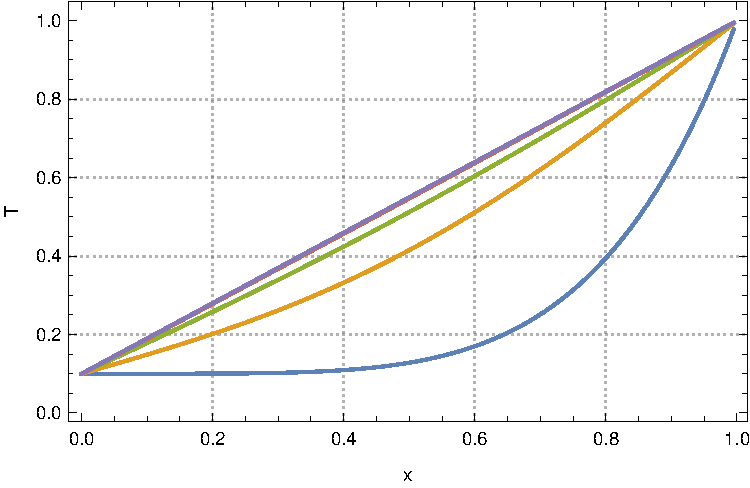
\includegraphics[width=\columnwidth]{figures/T_linear}
			\caption{Constant heat conduction test. Different colors denote the solution at uniform timesteps.}
			\label{linear_test}
		\end{figure}
		
		\begin{figure}[h!]
			\centering
			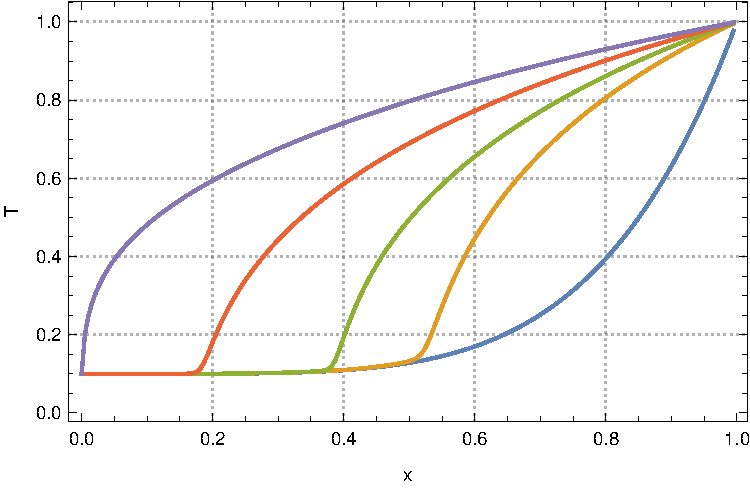
\includegraphics[width=\columnwidth]{figures/T_spitzer}
			\caption{Spitzer heat conduction test. Different colors denote the solution at uniform timesteps.}
			\label{spitzer_test}
		\end{figure}
		
		As predicted by the VNSA, there was no speedup possible using first-order EFD for both the constant and Spitzer conductivity.
		Any attempt to drive the solution faster would result in nyquist-frequency oscillations being amplified in regions of high temperature, which is a clear violation of the CFL condition.
	
		However, driving the parabolic and the hyperbolic solutions at the same timestep results in an RMS error of $1.18 \times 10^{-3}$, which is imperceptible at the scales of Figures \ref{linear_test} and \ref{spitzer_test}, indicating that the hyperbolic solution is working correctly.
	
	\section{Conclusion}
	
		It was disappointing that we were unable to achieve any speedup using the hyperbolic system along with first-order EFD. 
		\cite{A} was able to achieve over 100x speedup using the hyperbolic system, but they must've used a more sophisticated integration technique to prevent instabilities from forming. 
		We plan to investigate further using Runge-Kutta 2 methods to stabilize the solution.
		
		However we found the VNSA to be an effective method for determining the CFL condition for systems of PDEs.
		This method will be useful in future works for stabilizing explicit solvers.
			
	\bibliographystyle{apj}
	\bibliography{sources}
	
	\begin{acronym}
		\acro{MHD}{magnetohydrodynamics}
		\acro{DR}{dispersion relation}
		\acro{PDE}{partial differential equation}
		\acro{FD}{finite-difference}
		\acro{EFD}{explicit finite-difference}
		\acro{IFD}{implicit finite-difference}
		\acro{GPU}{graphics processing unit}
		\acro{LHS}{left-hand side}
		\acro{RHS}{right-hand side}
		\acro{CFL}{Courant-Friedrichs-Lewy}
		\acro{VNSA}{Von Neumann stability analysis}
		\acro{MPP}{massively-parallel processor}
	\end{acronym}
	
\end{document}